\chapter{调试通道总体设计与关键技术}

\section{总体设计}
	VxWorks的集成开发调试环境为Tornado,它使用串口和网口结合的方式来对目标机进行控制和数据传输,而目前对于大多数的设备而言都已经抛弃了串口,很多用于军事上的嵌入式设备都是专用设备,没有联网的需求,并不会配备网口,但是对于设备上产生的各种调试信息、日志信息都需要传输到我们的windows PC上来进行一个事后分析,因此我们需要设计一个新的调试通道来进行这些信息的传输,我们本次设计一个基于USB口转串口的底层驱动来实现该调试通道。本项目来源于中船重工在实际的生产环境当中的需求。
	调试通道的总体结构如\autoref{fig:debug-system-diagram}所示。
\begin{figure}[!h]
\centering
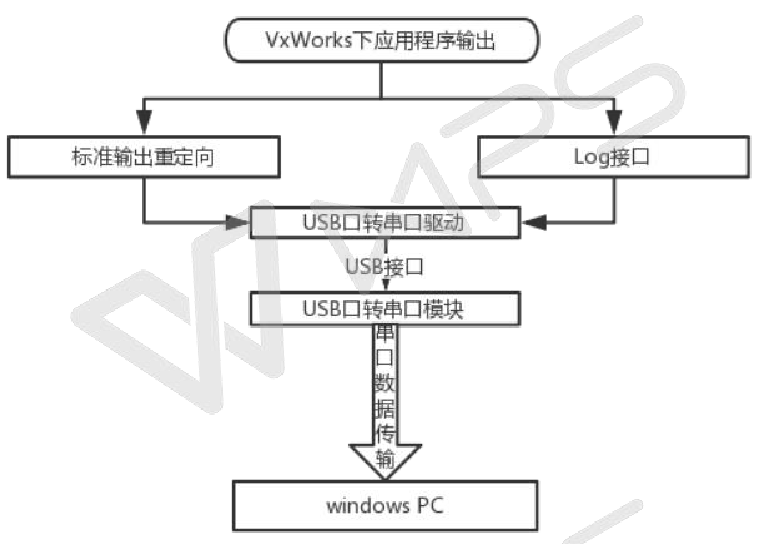
\includegraphics[width=.9\textwidth]{./graphics/debug-system-diagram.pdf}
\caption{调试通道整体结构图}\label{fig:debug-system-diagram}
\end{figure}
	
	整个调试通道主要分为两个模块:应用层的接口模块、USB口转串口模块。
	提供给应用层的接口模块负责将系统应用层的输出通过我们的USB口转串口驱动程序传输到windows PC机,输出的形式包括特定内容的格式化的输出和普通的重定向的输出,格式化的输出我们会使用自定义的Log接口进行格式控制,内容包含调试级别、调试信息所在的文件、调试信息所处的行号、输出该条调试信息的时间等。
	
	USB口转串口模块用于在VxWorks上实现一个USB口转串口驱动程序,负责将上层应用的信息传输到windows PC,主要包括驱动程序当中主要包含有驱动程序加载、卸载模块,设备的打开、关闭、读、写、控制模块。同时在驱动程序中还需要一个数据的管理模块,我们会使用循环缓冲区来管理数据。


\section{关键技术}

\subsection{VxWorks驱动开发}
	
	在VxWorks当中使用I/O子系统来管理设备驱动,I/O 子系统在整个VxWorks当中起着承上启下的作用,各种类型的设备都必须要向I/O子系统进行注册才能够被内核访问。I/O子系统维护着设备驱动中非常重的三个数据结构:系统设备表、系统驱动表、系统文件描述符表,设备驱动程序在初始化的时候会完成硬件设备寄存器的配置,同时也会向I/O子系统注册驱动和设备。在VxWorks中设备驱动的访问过程如下:
\begin{enumerate}
\item 使用open()函数打开一个名为devName的设备,此时VxWorks的I/O系统会在系统的设备表中寻找这个名为devName的设备项,并找到相应的驱动号; 
\item I/O系统在文件描述符当中保留一个文件描述符,然后在系统的设备驱动表中找到该设备的xxxOpen()函数,调用这个函数,并返回设备描述符的指针;
\item I/O系统将设备描述符的指针存储在文件描述符列表的Device ID中,同时将对应的设备驱动号存储在文件描述符的Driver Num项。最后I/O系统返回该描述符的索引(即fd);
\item 应用程序当中使用这个fd来调用read()、write()函数。系统会根据fd自动找到相应的设备驱动号,进而找到相应的驱动例程。 
\end{enumerate}

\subsubsection{VxWorks I/O 系统}
	通常操作系统为了平台的无关性都会为应用程序提供一套标准的接口,VxWorks也不例外,它为应用层的提供了接口函数creat()、open()、unlink()、remove()、close()、rename()、read()、write()、ioctl()、lseek()、readv()、writev()等,我们将其称作为标准I/O 库\cite{BSP开发人员指南}\cite{曹桂平2011VxWorks}。
	这样就可以通过调整底层驱动或者是接近驱动那部分的操作系统中间层来实现应用程序的通用性,提高应用层的开发效率,避免重复编码。通用操作系统(如Mac OS、Linux、Windows)中,通常会把这套接口从操作系统中独立出来,以标准库的形式存在,但是在VxWorks中它们是由系统的内核实现的,都位于ioLib.c文件下。VxWorks与通用操作系统有很大的一个不同点是:VxWorks不区分用户态和内核态,用户层可以直接对内核函数进行调用,而无需使用陷阱指令之类的机制,以及存在使用权限上的限制。因此VxWorks提供给应用层的接口无需通过外围库的方式,而是直接以内核文件的形式提供\cite{曹桂平2011VxWorks}。对于一般的设备而言,remove()接口是不需要实现的,\autoref{tab:IO接口函数表} 是七个驱动程序接口函数的简单描述。

\begin{table}[!h]
\centering
\begin{tabular}{|c|c|c|}
\hline
{\hei{接口名称}} & {\hei{函数原型}} & {\hei{描述}}\\ 
\hline
{open} & {open(filename,flags,mode)} & {打开一个新的或已存在的文件}\\
\hline
{create} & {create(filename,flags)} & {创建并打开一个新的文件}\\
\hline
{read} & {read(fd,\& buf,nBytes)} & {从文件中读取}\\
\hline 
{write} & {write(fd,\& buf,nBytes)} & {向文件中写入}\\ 
\hline
{ioctl} & {ioctl(fd,command,arg)} & {其他控制命令}\\
\hline
{close} & {close(fd)} & {关闭文件}\\
\hline
{remove} & {remove(filename)} & {移除文件}\\
\hline
\end{tabular}
\caption{IO接口函数表}\label{tab:IO接口函数表}
\end{table}
	
\subsubsection{系统设备表}
	系统设备表是VxWorks中为了管理系统上的所有设备而使用的一个链表。系统设备表在系统中的连接方式如\autoref{fig:VxWorks系统设备示意图}所示。wind内核规定每一个设备都必须使用一个DEV\_ HDR的结构来表示该设备,其定义如下:
\lstset{language=C}
\begin{lstlisting}
/*h/iosLib.h*/
typedef struct /*DEV_HDR - device header for all device structures*/ 
{ 
  DL_NODE node; /* device linked list node */ 
  short drvNum; /* driver number for this device */ 
  char * name;/* device name */ 
}DEV_HDR;  
\end{lstlisting}
VxWorks系统提供了一个设备的注册函数iosDevAdd( DEV\_ HDR *pDevHdr, char *name, int drvnum)来将设备添加到系统设备表当中,系统设备表在每次添加设备时就会增加一个节点,删除设备时就会减少一个节点,它会为open()、close()、remove()这三个函数提供文件与设备的连接,当应用程序执行这三个函数中的一个时,IO系统会通过文件名对设备链表中的项进行匹配,匹配的方式是最佳匹配,匹配成功之后就使用这个设备驱动进行其他的文件操作。


\begin{figure}[!h]
\centering
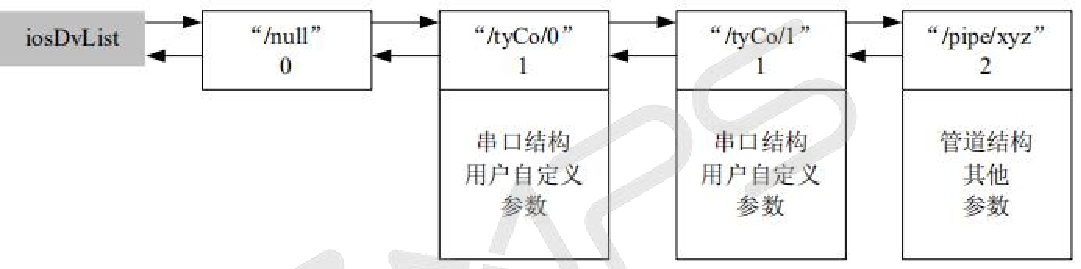
\includegraphics[width=1.0\textwidth]{./graphics/vxworks-device-link.pdf}
\caption{VxWorks系统设备示意图}\label{fig:VxWorks系统设备示意图}
\end{figure}

\subsubsection{系统驱动表}	
	系统驱动表用于管理当前注册到I/O子系统下的所有驱动,这些驱动可以是直接驱动硬件工作的驱动层,如一般的字符驱动,也可以是驱动中间层,如文件系统中间层,TTY 中间层,USB IO 中间层等。对于中间层驱动,下层硬件驱动将由这些中间层自身负责管理,而不再通过 IO 子系统。如串口底层驱动将通过 TTY 中间层进行管理,而不再通过IO子系统\cite{曹桂平2011VxWorks}\cite{罗国庆2003VxWorks}。
	
	系统驱动表底层的实现是一个数组,其中的每一个表项都是一个 DRV\_ ENTRY 类型的结构,该结构定义在 h/private/iosLibP.h文件当中,其定义如下:
\lstset{language=C}
\begin{lstlisting}
typedef struct /* DRV_ENTRY - entries in driver jump table */ 
{ 
  FUNCPTR de_create; 
  FUNCPTR de_delete; 
  FUNCPTR de_open; 
  FUNCPTR de_close; 
  FUNCPTR de_read; 
  FUNCPTR de_write; 
  FUNCPTR de_ioctl; 
  BOOL de_inuse; 
} DRV_ENTRY; 
\end{lstlisting}
DEV\_ ENTRY结构体实际上就是一个函数指针结构,结构中每个成员都指向一个完成特定功能的函数,这些函数与用户层提供标准函数接口一一对应\cite{VxWorksDriverAPI}\cite{Wind2003VxWorks}。成员 de\_ inuse 用以表示一个表项是否空闲。这个结构体中的函数指针实际指向的内容由驱动调用iosDrvInstall( FUNCPTR pCreate,FUNCPTR pDelete,FUNCPTR pOpen,FUNCPTR pClose,FUNCPTR pRead,FUNCPTR pWrite,FUNCPTR pIoctl)来提供。 


\subsubsection{系统文件描述符表}
	系统描述符表用于管理当前系统打开的所有文件描述符。其底层实现也是一个数组,文件描述符表的表项索引被用作文件描述符的ID(即open()函数返回值)。对于文件描述符有一点需要注意:标准输入,标准输出,标准错误输出虽然使用 0,1,2 三个文件描述符,但是可能在系统文件描述附表中只占用一个表项,即都使用同一个表项\cite{基于VxWorks的嵌入式实时系统设计}\cite{曹桂平2011VxWorks}。Vxworks 内核将 0,1,2 三个标准文件描述符与系统文件描述符表中内容分开进行管理。实际上系统文件描述符中的内容更多的是针对硬件设备,即使用一次 open 函数调用就占用一个表项。0,1,2 三个标准文件描述符虽然占用 ID 空间(即其他描述符此时只能从 3 开始分配),但是其只使用了一次 open 函数调用,此后使用 ioGlobalStdSet 函数对 open 返回值进行了复制\cite{嵌入式实时操作系统VxWorks及其开发环境Tornado}\cite{史小斌2003VxWorks}\cite{曹桂平2011VxWorks}。

系统文件描述符表中每个表项都是一个 FD\_ ENTRY 类型的结构,该结构定义在h/private/iosLibP.h 中,如下所示。
\lstset{language=C}
\begin{lstlisting}
typedef struct /* FD_ENTRY - entries in file table */ 
{ 
  DEV_HDR * pDevHdr;/* device header for this file */ 
  int value; /* driver's id for this file */ 
  char * name; /* actual file name */ 
  int taskId; /* task to receive SIGIO when enabled */ 
  BOOL inuse; /* active entry */ 
  BOOL obsolete; /* underlying driver has been deleted */ 
  void * auxValue;/* driver specific ptr, e.g. socket type */ 
  void * reserved; /* reserved for driver use */ 
} FD_ENTRY; 
\end{lstlisting}

用户程序每调用一次 open 函数,系统文件描述符表中就增加一个有效表项,直到数组满,此时 open函数调用将以失败返回。表项在表中的索引偏移 3 后作为文件描述符返回给用户,作为接下来其他所有操作的文件句柄。	
	
\subsection{VxWorks 中的通信机制}
	
	wind内核提供了三种任务间通信机制(不包括信号机制):信号量,消息队列,管道。这三种机制都是使用的共享物理内存机制,这块共享的内存是由内核进行管理的,任务必须通过内核提供的接口函数进行访问,这种保护和管理机制使任务间通信安全有序的进行。

\begin{enumerate}
	\item \textbf{信号量}
	
	信号量的主要用途是互斥和同步。基于各种资源的不同使用方式,VxWorks信号量机制具体的提供了三种信号量:通用信号量;互斥信号量;资源计数信号量。通用信号量既可用于同步也可用于资源计数,此时资源数通常为 1(当资源数为 1 时,也可以称之为互斥)。互斥信号量针对在使用过程中一些具体问题(如优先级反转)做了优化,更好的服务于任务间互斥需求;资源计数信号量用于资源数较多,同时可供多个任务使用的场合。
	
	VxWorks中信号量是一种指向semaphore结构的指针,其定义如下所示:
\lstset{language=C}
\begin{lstlisting}
typedef struct semaphore
{
  OBJ_CORE objCore;/*对象管理*/
  UINT8 semType; /*信号量类型*/
  UINT8 options; /*信号量选择*/
  UINT16 recurse; /*信号量重复获取计数器*/
  Q_HEAD qHead; /*阻塞的任务队列头*/
  union{
	UNIT count;/*当前状态*/
	struct windTcb *owner;  
  }state;
  EVENTS_RSRC events;/*VxWorks事件*/
}SEMAPHORE;
\end{lstlisting}
	
	\item \textbf{消息队列}
	
	消息队列内核实现上实际是一个结构数组,数组大小和数组中元素的容量在创建消息队列时被确定。消息队列是 Vxworks 内核提供的任务间传递较多信息的一种机制,不过这种机制存在的很大的局限性,即每个消息的最大长度是固定的。Vxworks内核提供的消息机制在创建消息队列时就必须指定单个消息的最大长度以及消息的数量,在消息队列成功创建后,这些参数都是固定不变的。
	
	\item \textbf{管道}
	
	管道相比消息队列提供了一种更为流畅的任务间信息传递机制。消息队列必须将信息分批打包,而且对于每个消息的大小存在限制,而管道可以像文件那样进行读写,是一种流式消息机制。管道通常分为两种:命名管道和非命名管道。任务间通信使用的一般都是命名管道。非命名管道使用在线程意义上,如父子进程,进程关系密切,且某些变量存在继承关系,如文件描述符,一般无法使用在两个执行路线完全不同的任务之间。
\end{enumerate}\\		
\textbf{任务间特殊的通信机制--信号:} 信号用于通知一个任务某个事件的发生。Vxworks中的信号处理机制有些特别之处,当一个任务接收到一个信号时,在这个任务下一次被调度运行之时进行信号的处理(即调用相关信号处理函数)。事实上,由于 Vxworks 在退出内核函数时都会进行任务调度,故一个任务,无论是否是当前执行任务,都将在被调度运行时执行信号的处理。通用操作系统上对于某些信号将不允许用户修改其默认处理函数,如 SIGKILL,SIGSTOP,然而 VxWorks 操作系统中可以对任何信号的处理函数都可以进行更换。




\subsection{USB技术}
	USB(Universial Serial Bus,通用串行总线)是这十几年来应用在PC领域的最新型的接口技术,出现的契机是为了为了解决日益增加的PC外设与有限的主板插槽之间的矛盾,其实现是由一些PC大厂商(Microsoft、Intel等)定制出来的,自从1995年在Comdex上展出以来至今已广泛地被各个PC厂家所支持。目前已经在各类外部设备中都广泛的采用USB接口。USB接口标准目前有三种:USB1.1,USB2.0和USB3.0。USB接口应用如此的广泛是由其独特和实用的特性决定的。

\noindent USB规范规定了USB传输的四种方式,每种方式有各自的用途\cite{USB总线接口开发指南}:
\begin{itemize}
\item \hei{控制传输}:控制传输是每一个设备必须要具有的传输方式,也是四种传输方式中过程最复杂的部分,他使得主机能够从设备列出的范围中读取和选择配置和其他设置,也能够发送自定义请求来为任何目的而发送和接收数据,在配置和列举的过程中起到重要的作用。
\item \hei{批量传输}:批量传输是为了处理传输速率不是很关键的情况,一般用于打印机和扫描仪。
\item \hei{中断传输}:中断传输是为了那些要快速实现主机和设备的交互而准备的,比如适用于鼠标和键盘。
\item \hei{等时传输}:等时传输用于必须要按照一个常数传输数据的情况,比如一个需要被实时播放的视频/音频数据流。
\end{itemize}\\
所有的传输都是由事务组成,事务又由包组成,而包包含一个包识别器(PID)、CRC和其他的信息\cite{USB大全}。

	USB的体系结构如\autoref{fig:USB体系结构}所示
\begin{figure}[!h]
\centering
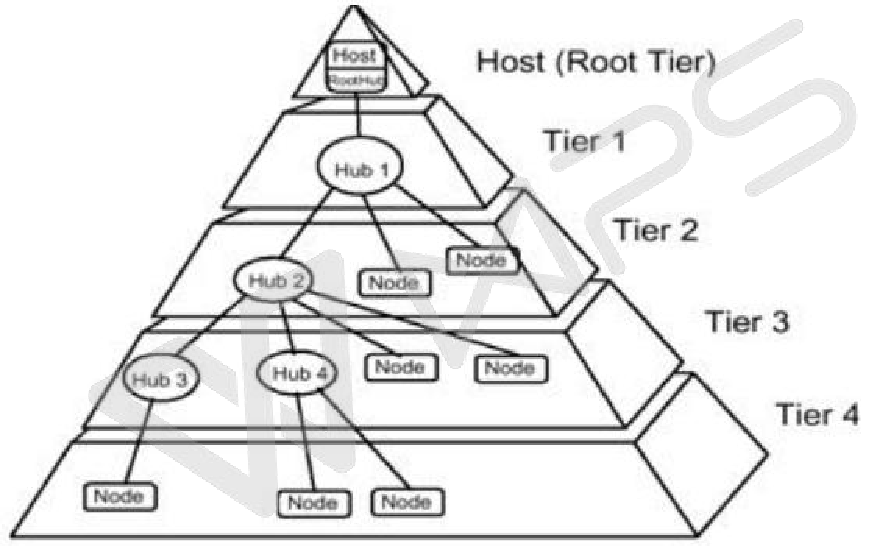
\includegraphics[width=1.0\textwidth]{./graphics/usb-structure.pdf}
\caption{USB总线拓扑结构}\label{fig:USB体系结构}
\end{figure}

	USB的物理层拓扑为星型结构,包括三个部分:USB主机(Host)、USB集线器(Hub)、USB设备(Device)。
	
\begin{enumerate}
\item \textbf{USB主机}

	USB的体系结构只允许系统中有一个主机,主计算机系统的USB接口称之为USB主控制器。主控制器可以是硬件、固件或软件的联合体,其控制着总线上所有USB设备和所有集线器的数据通信过程。所有的数据传输都是由USB的主机端发起的,而且如果USB主机嵌入在一个计算机系统中,在数据的传输过程中也不需要计算机的CPU参与传输工作。USB主机通常具有以下的功能:
	\begin{itemize}
	\item 检测USB设备的插拔动作(通过根集线器来实现)
	\item 管理 USB 主机和USB设备之间的控制流
	\item 管理USB主机和USB设备之间的数据流
	\item 收集USB主机的状态和USB设备的动作信息
	\end{itemize}
\item \textbf{USB集线器}
	
	根集线器是集成在主机系统当中的一个特殊集线器,他可以提供一个或者跟多的接入口。在即插即用的USB体系结构当中,集线器是一种很重要的设备。其极大的简化了USB的复杂性,而且以很低的价格和易用性提供了设备的健壮性,集线器的最大的连接能力是127。

\item \textbf{USB设备}

	USB设备是USB总线系统的重要组成部分,它们以从属的方式与USB主机进行通信,并受USB主机的控制。USB主机端提供的协议软件通过和USB设备通信获得设备的信息,并给设备提供驱动程序,相比USB主机而言,USB设备只能够被动的应答,按照USB主机的要求接受或者发送数据。USB设备通过以下的属性来完成主机的要求:
	\begin{itemize}
	\item \textbf{描述符}\\
	USB协议为USB设备定义了一套描述设备功能和属性的固定结构的描述符,通过这些描述符向USB主机汇报设备的各种属性,主机通过对这些描述符的访问对设备进行识别、配置并为其提供相应的客户端驱动程序。典型的描述符一般由USB标准描述符和USB类描述符,或者由USB标准描述符和USB厂商特定描述符组成。运行于USB协议栈上层的客户端驱动程序通过这些信息正确的访问设备并与其进行通信,以实现即插即用的目的。
	\item \textbf{类}\\
	USB协议支持许多的外围设备,为了正确的驱动这些设备,USB主机端要为这些设备提供符合USB协议的驱动程序,称为客户端驱动。同时为了避免客户端程序过多,协议通过归纳将设备划分为不同的设备类,把功能相近的设备归为一类,主机端只需要提供类驱动程序便可以驱动大多数的USB设备。	
	\item \textbf{功能(Function)/接口(Interface)}\\
	在USB协议中,Function被定义为具有某种能力的设备,即相当于传统的单一功能设备。随着USB设备应用的发展,物理上几种不同的Function可以组成一台设备,只要设备的接口具有某种独立的能力,就称为一个Function。Function是从功能角度来说的,从设备的角度来说,它又被称为Interface。
	\item \textbf{端点(Endpoint)}\\
	端点层的各个子模块是USB设备与USB主机逻辑上的数据传输的最基本单元,即最基本的通信点,因而端点层的每一个逻辑模块被称为端点(Endpoint)。每一个端点都关联一个相应的端点号和数据传输方向(IN/OUT)。具有相同端点号和不同传输方向的通信点表示不同的端点,端点0被USB规范保留用作设备枚举和配置过程中的数据传输端点,与端点0对应的管道是默认管道,设备的所有端点共享端点0。在一个USB系统当中,USB主机对特定设备功能的访问是通过使用不同的端点号,否则,USB主机将不能对相应的设备进行正确的访问。由于在系统运行时,不同的设备配置有着互斥性,因而在不同的配置描述中,端点号是可以重复的。
	\item \textbf{管道}\\
	设备端点与USB主机所形成的具有特定数据传输特性(如数据传输格式、传输带宽、传输方向等)的数据通道,被称为管道。管道的物理介质就是USB系统中的数据线。端点层的USB设备与USB主机之间的数据传输都是基于管道进行的。
	\item \textbf{设备地址}\\
	USB主机的客户端驱动程序通过描述符来区分不同的设备,而USB主机控制器通过设备地址来区分设备。设备地址共有7位,表示理论上系统可以同时连接127个USB设备,但是在实际中,由于USB总线带宽的限制,这么多设备不可能同时的工作。USB主机负责为USB系统中的设备分配不同的设备地址,用来表示哪个设备的同时还要指名设备的端点号,表示使用哪个管道。
	\end{itemize}	
	
\end{enumerate}

	一个主机和设备的连接需要一些列的层次和实体之间的交互,USB接口层在主机和设备间提供物理、信号包的关联,USB设备层表示USB系统程序实现对一个设备进行的总的USB操作,功能层适当匹配的客户服务程序层提供附加的功能给主机。设备和功能层当中各自有逻辑通信,但是实际的USB数据传输是通过USB总线接口层来实现的\cite{USB开发手册}\cite{圈圈教你玩USB}。


\section{本章小结}
	本章重点介绍了本次的VxWorks调试通道的整体架构,并介绍了介绍了各个部分的设计方案,最后介绍了在本次的设计当中所需要使用关键技术和所需了解的重要知识,主要包括VxWorks下的驱动开发必须的结构、驱动中所需使用的VxWorks的通信机制、缓冲区技术、USB技术。下面将要讨论VxWorks下的调试通道的详细的设计细节和具体的实际机制。

























